% Title: Report LaTex File: Hardware Development
% Auther: DC Eksteen
% Student Number: 22623906
% Contact: 22623906@sun.ac.za
% Date: 2022/09/14
% Version: 2.0

\chapter{Hardware Development}

\color{red} % Comment if section finalized

% Section overview: Hardware development.
For the project, hardware was developed with the aim of achieving the objectives shown in \ref{tab:devgoals} below:

\begin{table}[H]
	\color{red} % Comment if section finalized
	\renewcommand{\arraystretch}{1.2}
	\centering
	\caption{Objectives of Hardware Development}
	\begin{tabularx}{\textwidth}{p{2cm} >{\raggedright}p{5cm} >{\raggedright\arraybackslash}X}
		\toprule
		Outcome Number & Description          & Required Outcome            \\
		\midrule
		H 1            & Versatile Usage      & Design for adaptable length \\
		H 2            & Wide Operating Range & Adequate Braking Force      \\
		H 3            & Outcome 3            & Description                 \\
		H 4            & Outcome 4            & Description                 \\
		\bottomrule
	\end{tabularx}
	\label{tab:devgoals}
\end{table}

\color{black}
\newpage

\section{Expected Operating Conditions}
\color{red} % Comment if section finalized

The expected operating range of a cyclist on the trainer will typically range between \SI{10}{\kilo\meter\per\hour} and \SI{60}{\kilo\meter\per\hour}.

Typical bicycle measurements are as seen in Table \ref{tab:bikesize} below.

\begin{table}[H]
	\color{red} % Comment if section finalized
	\renewcommand{\arraystretch}{1.2}
	\centering
	\caption{Summery of Typical Bicycle Dimensions}
	\begin{tabularx}{\textwidth}{p{1.4cm} >{\raggedright}p{5cm} >{\raggedright\arraybackslash}X}
		\toprule
		Size & Wheel Diameter         & Wheelbase              \\
		\midrule
		1    & \SI{115}{\milli\meter} & \SI{115}{\milli\meter} \\
		2    & \SI{115}{\milli\meter} & \SI{115}{\milli\meter} \\
		3    & \SI{115}{\milli\meter} & \SI{115}{\milli\meter} \\
		13   & \SI{115}{\milli\meter} & \SI{115}{\milli\meter} \\
		\bottomrule
	\end{tabularx}
	\label{tab:bikesize}
\end{table}

\begin{figure}[H]
	\begin{center}
		\includegraphics[width=0.5\textwidth]{SpeedCalculations.jpg}
		\caption{Rotational Speed of Roller Size Comparison}
		\label{fig:speedCalc}
	\end{center}
\end{figure}

\color{black}
\newpage

\section{Eddy Current Brake Design}
\color{red} % Comment if section finalized

The Eddy Currents in the Aluminium disc will be:
\[
	\acs{I}_e = \frac{\acs{condDisk} \acs{B} \acs{v}}{2}
\]
The eddy currents within the disc is then:
\[
	di = \frac{\acs{I}_e}{2 \pi} d\acs{theta}
\]
Using Ampere's Law, the force on an element at length l is then:
\[
	d\acs{F} = \acs{B} \, di \, dl
\]
\[
	d\acs{T} = l \, d\acs{F}
\]
Thus, combining all these, we get:
\[
	d\acs{T} = \frac{\acs{B} \, \acs{I}_e}{2 \pi} \, l \, d\acs{theta} \, dl
\]
By integrating, we get:
\[
	\int_{0}^{R} \int_{0}^{2 \pi} \frac{\acs{B} \, \acs{I}_e}{2 \pi} \, l \, d\acs{theta} \, dl
\]
\[
	\acs{T} = \frac{\acs{condDisk}\acs{B}^2\acs{omega}_n R^2}{6}
\]

\begin{figure}[H]
	\begin{center}
		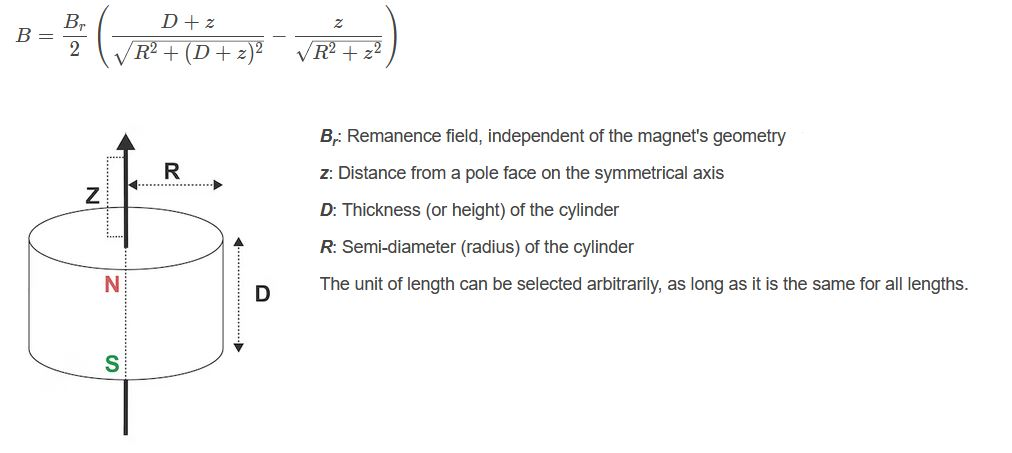
\includegraphics[width=0.8\textwidth]{Bfieldcalc.jpg}
		\caption{Magnetic Flux Density of Disc Magnet}
		\citep[Addapted from][]{Supermagnete:2010}
		\label{fig:B0}
	\end{center}
\end{figure}

\begin{figure}[H]
	\begin{center}
		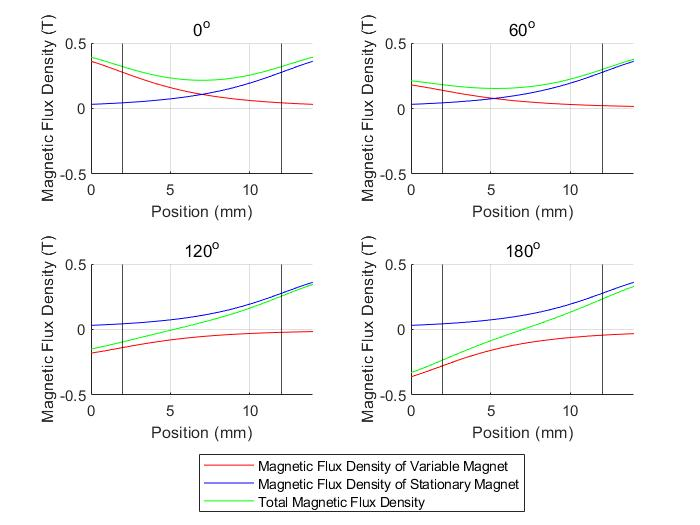
\includegraphics[width=\textwidth]{FluxDensityPhases.jpg}
		\caption{Magnetic Flux Density as Phase Changes}
		\label{fig:fluxD0}
	\end{center}
\end{figure}


$\frac{0.65\,{\left(0.001\,x-0.014\right)}}{\sqrt{{{\left(0.001\,x-0.014\right)}}^2 +0.000056249999999999998460432915070584}}-\frac{0.65\,{\left(0.001\,x-0.019\right)}}{\sqrt{{{\left(0.001\,x-0.019\right)}}^2 +0.000056249999999999998460432915070584}}$

\color{black}